\documentclass[11pt,a4paper]{article}

\usepackage{listings}
\usepackage{parskip}
\usepackage{tikz}
\usepackage{hyperref}
\usepackage{tabularx}
\usepackage{fullpage}

%% Do not use monospaced fonts for URLs
\urlstyle{same}

%% Initializing tikz and nodes we need.
\usetikzlibrary{calc, chains, decorations.pathreplacing}

%% Define a document shaped node.
\makeatletter
  \pgfdeclareshape{document}{
    \inheritsavedanchors[from=rectangle] % this is nearly a rectangle
    \inheritanchorborder[from=rectangle]
    \inheritanchor[from=rectangle]{center}
    \inheritanchor[from=rectangle]{north}
    \inheritanchor[from=rectangle]{south}
    \inheritanchor[from=rectangle]{west}
    \inheritanchor[from=rectangle]{east}
    % ... and possibly more
    \backgroundpath{% this is new
        % store lower right in xa/ya and upper right in xb/yb
        \southwest \pgf@xa=\pgf@x \pgf@ya=\pgf@y
        \northeast \pgf@xb=\pgf@x \pgf@yb=\pgf@y
        % compute corner of ‘‘flipped page’’
        \pgf@xc=\pgf@xb \advance\pgf@xc by-10pt % this should be a parameter
        \pgf@yc=\pgf@yb \advance\pgf@yc by-10pt
        % construct main path
        \pgfpathmoveto{\pgfpoint{\pgf@xa}{\pgf@ya}}
        \pgfpathlineto{\pgfpoint{\pgf@xa}{\pgf@yb}}
        \pgfpathlineto{\pgfpoint{\pgf@xc}{\pgf@yb}}
        \pgfpathlineto{\pgfpoint{\pgf@xb}{\pgf@yc}}
        \pgfpathlineto{\pgfpoint{\pgf@xb}{\pgf@ya}}
        \pgfpathclose
        % add little corner
        \pgfpathmoveto{\pgfpoint{\pgf@xc}{\pgf@yb}}
        \pgfpathlineto{\pgfpoint{\pgf@xc}{\pgf@yc}}
        \pgfpathlineto{\pgfpoint{\pgf@xb}{\pgf@yc}}
        \pgfpathlineto{\pgfpoint{\pgf@xc}{\pgf@yc}}
    }
}
\makeatother

%% Tikz node and path shapes that are used for figures.
\tikzset{
    doc/.style={
        draw, 
        align=center, 
        color=black, 
        shape=document,
        minimum width=3.5em, 
        minimum height=5em, 
        shape=document, 
        inner sep=2ex,
        font=\ttfamily,
        on chain},
    action/.style={
        rectangle, 
        draw=black, 
        text centered, 
        rounded corners, 
        text width=7em, 
        minimum height=2em,
        on chain},
    tuborg/.style={
        decorate},
    tubnode/.style={
        midway,
        right=4pt}
}

%% The formatting of code.
\lstset{
    basicstyle=\ttfamily,
    xleftmargin=15pt,
    basewidth={.48em}
}

%% A shortcut for emphasising code identifiers in text.
\newcommand{\tc}{\texttt}

\title{sth \\ A Simplethon compiler}
\date {Version 0.1}

\begin{document}
 \maketitle
 \section{Introduction}

\begin{figure}[h!]
    \begin{center}
        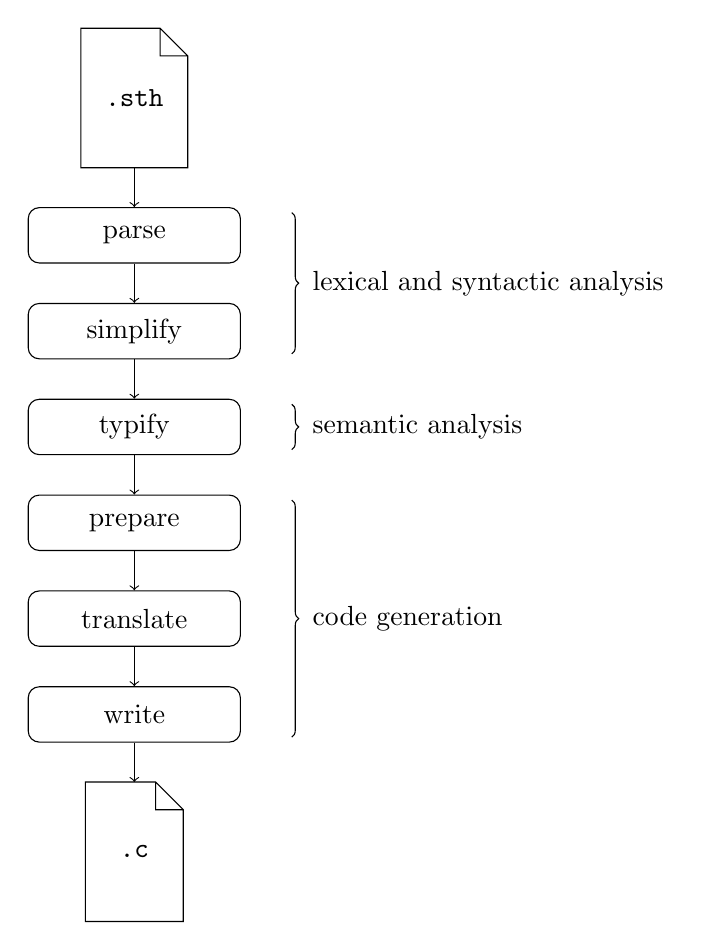
\begin{tikzpicture}[node distance=.5cm, start chain=going below]

    \node (sthsource)   [doc]     {.sth};
    \node (parse)       [action]  {parse};
    \node (simplify)    [action]  {simplify};
    \node (typify)      [action]  {typify};
    \node (prepare)     [action]  {prepare};
    \node (translate)   [action]  {translate};
    \node (write)       [action]  {write};
    \node (csource)     [doc]     {.c};

    \draw[->] (sthsource) -- (parse);
    \draw[->]     (parse) -- (simplify);
    \draw[->]  (simplify) -- (typify);
    \draw[->]    (typify) -- (prepare);
    \draw[->]   (prepare) -- (translate);
    \draw[->] (translate) -- (write);
    \draw[->]     (write) -- (csource);

    \draw[tuborg, decoration={brace}] let \p1=(parse.north), \p2=(simplify.south) in
        ($(2, \y1 - 2)$) -- ($(2, \y2 + 2)$) node[tubnode] {lexical and syntactic analysis} ;

    \draw[tuborg, decoration={brace}] let \p1=(typify.north), \p2=(typify.south) in
        ($(2, \y1 - 2)$) -- ($(2, \y2 + 2)$) node[tubnode] {semantic analysis} ;

    \draw[tuborg, decoration={brace}] let \p1=(prepare.north), \p2=(write.south) in
        ($(2, \y1 - 2)$) -- ($(2, \y2 + 2)$) node[tubnode] {code generation} ;

\end{tikzpicture}

    \end{center}
    \caption{Workflow}
\end{figure}
  

 \input{ast.py.tex}
 \input{parser.py.tex}
\end{document}
